\documentclass[11pt]{article}
\usepackage[T1]{fontenc}
\usepackage{lmodern,amsmath,amssymb,microtype,tikz}
\usepackage[margin=0.88in]{geometry}
\usepackage[colorlinks=true,urlcolor=blue!55!black]{hyperref}
\newcommand{\R}{\mathbb R}
\newcommand{\one}{\mathbf 1}
\newcommand{\res}{\mathcal R}
\newcommand{\linf}{\infty}
\hypersetup{pdftitle={How precisely must one measure resistance to recover every missing edge?},pdfauthor={Wentao Li}}
\title{How precisely must one measure resistance\\ to recover every missing edge?}
\author{Wentao Li\\\small Prepared with assistance from OpenAI GPT-6.2 Astra}
\date{November 27, 2026}
\begin{document}
\maketitle
\begin{abstract}
In a connected simple graph on $n$ labeled vertices, suppose the adjacency matrix is given except on $k$ unordered pairs. Query the effective resistance once on each missing pair. Adversarial additive error strictly below $1/n^2$ per reading still permits exact recovery in polynomial bit time. At error $1/[n(n-2)]$, two graphs already give compatible readings on four specified pairs. Thus the leading constant in the worst-case noise radius for this measurement scheme is one. The algorithm works for any explicitly given finite alphabet of nonnegative rational conductances. It uses a piecewise quadratic penalty that preserves convexity and makes each admissible conductance stable under measurement error.
\end{abstract}

\section*{The question and the model}
Bennett, Black, Nayyeri and Warton first posted their graph-inference problem in 2025. Their ALT 2026 paper asks in Section 1.1 whether graph completion can combine a subquadratic number of queries in $k$ with polynomial running time. Theorem 37 gives exact recovery by enumerating a finite alphabet after $k$ queries. Section 6.3 and Theorem 39 identify the weighted solution as the minimizer of a log-determinant objective and discuss polynomial convergence of numerical optimization. We use that objective and prove a discrete decoding guarantee with an explicit noise radius and a rational bit-complexity bound. Earlier, Hoskins, Musco, Musco and Tsourakakis studied inference from partial and noisy resistance data in a different observation model.

Let $U$ be the $k$ missing unordered pairs. All other conductances are known nonnegative rationals. The unknown conductance on each pair belongs to the same explicitly listed rational alphabet $A=\{a_0<\cdots<a_s\}\subset[0,W]$, and all known conductances are at most $W$. Zero represents an absent edge. The true graph is connected. Assume $n\ge2$, $k\ge1$, $s\ge1$, since the other cases require no inference. Put $\Delta=\min_i(a_{i+1}-a_i)>0$. For every $e\in U$, the one query supplies a rational $y_e$ with $|y_e-\res_e(w)|\le\eta$, where $w$ denotes the vector of true conductances on $U$.

\paragraph{Exact decoding theorem.}
If $\eta<\Delta/(nW)^2$, a deterministic algorithm recovers $w$ in polynomial bit time from these $k$ readings. The time is polynomial in $n,k$ and the encoding lengths of the rational data including a promised rational error bound $\eta$. In the unweighted case take $A=\{0,1\}$ and $W=1$. In particular, exact readings suffice for polynomial-time exact completion.

\section*{A convex objective with a corner at each allowed weight}
For $e=ij$ write $b_e=e_i-e_j$. Let $L(x)$ be the graph Laplacian for the known weights and proposed unknown weights $x$. Set $M(x)=L(x)+\one\one^T/n$. On the convex part of $[a_0,a_s]^k$ giving connected graphs, $M$ is positive definite and $\res_e(x)=b_e^TM(x)^{-1}b_e$. Put
\[
 f(x)=y^T x-\log\det M(x),\qquad \lambda=(nW)^{-2}.
\]
The gradient of $f$ has entries $y_e-\res_e(x)$. For a direction $d$ put $B=\sum_{e\in U}d_eb_eb_e^T$. Its two off-diagonal entries on $e$ are $-d_e$. On $\one^\perp$, $M(x)\preceq nW I$ by comparison with the complete graph of conductance $W$, and $B\one=0$. Twice differentiating gives
\[
 D^2f(x)[d,d]=\|M(x)^{-1/2} B M(x)^{-1/2}\|_F^2
 \ \ge\ (nW)^{-2}\|B\|_F^2\ \ge\ 2\lambda\|d\|_2^2 .
\]
The first bound follows by diagonalizing $M$ on $\one^\perp$. Consequently $f(x)-\lambda\sum_e x_e^2$ is convex on the box wherever $M\succ0$.

Between two consecutive levels $a,b$ define $p(t)=(t-a)(b-t)$. This continuous function vanishes at the allowed levels. The function $p(t)+t^2$ is the linear interpolant of $t^2$ on $A$, with successive slopes $a+b$ increasing. It follows that
\[
                 F(x)=f(x)+\lambda\sum_{e\in U}p(x_e)
\]
is convex. At an allowed level, moving a distance $h$ to an allowed side has first-order penalty equal to $|h|$ times the gap on that side. At the true $w$ the gradient error of $f$ has each entry bounded by $\eta$. Convexity and the one-sided directional derivative at $w$ therefore give, for every connected feasible $x$,
\[
               F(x)-F(w)\ge c\|x-w\|_1,\qquad c=\lambda\Delta-\eta>0. \tag{1}
\]
This identifies the exact discrete optimum under noise of either sign on every query. The bound does not shrink with $k$.

\section*{Polynomial-time recovery with rational cuts}
We give the bit argument because uniqueness or numerical convergence alone does not specify how to recover an exact alphabet entry on the boundary. At a candidate alphabet vector $v$, first check connectivity. If connected, let $g_e=y_e-\res_e(v)$. For each level $v_e$ with a previous level $a$, check $g_e-\lambda(v_e-a)\le0$. If it has a next level $b$, check $g_e+\lambda(b-v_e)\ge0$. These are the left and right optimality inequalities of a convex function on a box. They are necessary and sufficient, since all feasible directional derivatives are sums of the corresponding one-coordinate derivatives. Connectivity holds on a relative neighborhood of a connected point. Equation (1) makes $w$ the only candidate that passes.

Start the rational central-cut ellipsoid method in a ball about the origin of radius $k(W+1)$. At a center outside the box, cut through the center along an offending coordinate, retaining the box. At a disconnected center inside the box, choose one connected component. Cut in the direction of increasing total unknown conductance across its boundary. The crossing sum is zero at the center and is positive throughout the connected feasible region. For a connected center $x$, round each coordinate to its nearest alphabet level, breaking ties arbitrarily, and test the resulting candidate as above. On success return it. Otherwise $\|x-w\|_\infty\ge\Delta/2$, and (1) gives $F(x)-F(w)\ge c\Delta/2$. Retain the central halfspace $g^T(z-x)\le0$ for any subgradient $g$ of $F$ on the box at $x$. A rational subgradient is computed from $y_e-\res_e(x)+\lambda(a+b-2x_e)$ using either incident interval $[a,b]$ at a level. This halfspace retains all points with cheaper objective. At an unsuccessful center the subgradient cannot vanish.

To bound the number of cuts, put $D=a_s-a_0$ and consider the ball of radius $D/4$ about the constant midpoint vector of the box. Every vector $u$ there satisfies $u_e\ge w_e/4$, so $M(u)\succeq M(w)/4$. Hence
\[
 F(u)-F(w)\le H,\qquad H=1+2n+kD(\|y\|_\infty+\lambda D).
\]
Here the determinant term costs at most $n\log4$, and $0\le p(t)\le D^2/4$. Contract that ball toward $w$ by the factor $\theta=\min(1/2,c\Delta/(4H))$. Convexity gives a ball of radius $\theta D/4$ of connected feasible points with cost at most $F(w)+c\Delta/4$. Every unsuccessful cut retains it. The central-cut ellipsoid volume bound, with its usual polynomial-bit rounding, forces success in polynomially many iterations in $k$ and $\log(1+4k(W+1)/(\theta D))$. In dimension one ordinary interval bisection gives the same conclusion.

All cuts, candidate tests and constants above use rational arithmetic. Graph connectivity uses the positive-conductance support. Resistance evaluations use rational linear solves on $M$, whose output lengths are polynomial in the bit size of the center and graph by determinant bounds. The rounded rational ellipsoid algorithm keeps centers of polynomial bit length. Exact oracle responses for rational input weights also have polynomial bit length, by the same determinant bounds. This proves the stated complexity without evaluating a logarithm in the algorithm.

\section*{A four-edge ambiguity and the sharp leading constant}
For $n\ge4$ form $G$ and $H$ by deleting from $K_n$ the matchings $\{12,34\}$ and $\{13,24\}$ respectively. Let $U$ be these four pairs. If $C$ is the Laplacian of a matching then $C^2=2C$. On $\one^\perp$ the inverse Laplacian of the graph after deletion is
\[
            (nI-C)^{-1}=I/n+C/[n(n-2)].
\]
For a queried pair $e$, $b_e^TCb_e$ is four if it is a deleted matching edge and two if it connects different matched pairs. Thus on \emph{each} queried pair the readings differ by exactly $2/[n(n-2)]$. Their midpoint transcript has error $1/[n(n-2)]$ for both graphs. No decoder receiving these four measurements can always identify the graph at that error.
\begin{center}
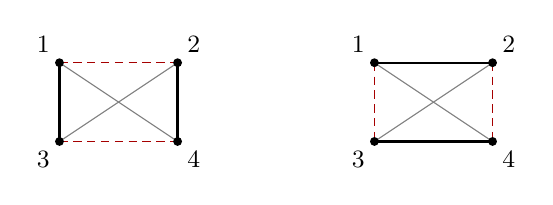
\begin{tikzpicture}[x=1cm,y=1cm, every node/.style={font=\small}]
\foreach \offset/\kind in {0/0,4.0/1}{
\begin{scope}[xshift=\offset cm]
\coordinate (p1) at (0,1); \coordinate (p2) at (1.5,1);
\coordinate (p3) at (0,0); \coordinate (p4) at (1.5,0);
\draw[gray] (p1)--(p4) (p2)--(p3);
\ifnum\kind=0 \draw[thick] (p1)--(p3) (p2)--(p4); \draw[densely dashed,red!65!black] (p1)--(p2) (p3)--(p4);
\else \draw[thick] (p1)--(p2) (p3)--(p4); \draw[densely dashed,red!65!black] (p1)--(p3) (p2)--(p4); \fi
\foreach \i/\pos in {1/above left,2/above right,3/below left,4/below right}{\fill (p\i) circle (1.6pt) node[\pos] {$\i$};}
\end{scope}}
\end{tikzpicture}\\
{\small Dashed pairs are absent. All pairs involving a vertex outside the figure are present.}
\end{center}
Writing $r_n$ for the supremum of the uniformly decodable error radii for this specified measurement scheme, the two theorems give
\[
            1/n^2\le r_n\le 1/[n(n-2)],\qquad \lim_{n\to\infty} n^2 r_n=1 .
\]
The upper bound concerns querying the missing pairs themselves. It leaves other choices of queried pairs unrestricted by this example.

\section*{Sources and status}
\begin{itemize}
\item H. Bennett, M. Black, A. Nayyeri and E. Warton, \href{https://arxiv.org/abs/2502.18350}{Graph Inference with Effective Resistance Queries, 2025 preprint}; \href{https://proceedings.mlr.press/v313/warton26a.html}{ALT 2026}, Sections 1.1 and 6.2--6.3.
\item J. Hoskins, C. Musco, C. Musco and C. Tsourakakis, \href{https://proceedings.neurips.cc/paper_files/paper/2018/file/2f25f6e326adb93c5787175dda209ab6-Paper.pdf}{Inferring Networks From Random Walk-Based Node Similarities}, NeurIPS 2018.
\item M. Gr\"otschel, L. Lov\'asz and A. Schrijver, \href{https://www.mpi-inf.mpg.de/fileadmin/inf/d1/ellipsoid-lovasz.pdf}{Geometric Algorithms and Combinatorial Optimization}, Section 3.2, rational central cuts.
\end{itemize}
Research draft. The source authors supply the log-determinant formulation. The discrete noise guarantee, its asymptotically matching obstruction and the exact bit algorithm are the contributions claimed here. Independent mathematical and priority review are pending.
\end{document}
